\chapter{Introduction}
\label{ch:intro}
\fancyhead[L]{Introduction}
\fancyhead[C]{}
\fancyhead[R]{}
\fancyfoot[C]{\thepage}

\section{Brief introduction to the thesis}
Since antiquity, when ancient peoples like the Olmecs, Chinese and Greeks \citep{Carlson1975,Evans1977,May1981} discovered the strange properties of lodestones (rocks composed of magnetite and hematite), the magnetism of rocks has marvelled human imagination. The first modern treatise on a scientific subject was William Gilbert's \emph{De Magnete}, first published in 1600. It is unquestionable, then, that magnetism lies at the heart of modern science.\par

In the first half of the XX century, scientific studies \citep{Koenigsberger1938,Thellier1938,Nagata1943} of how rocks acquired and retained magnetisations gave rise to the discipline of rock magnetism. Knowledge of rock magnetism has been behind some of the deepest breakthroughs in our knowledge of the workings of our planet, e.g., continental drift. Today, insights gained from rock magnetism are used to study the history of Earth's and the Sun's magnetic field (palaeomagnetism) \citep{Dunlop} as well as palaeoclimates (environmental magnetism) \citep{Evans}, among other applications in Earth and planetary science.\par

Airborne magnetic surveys over oil fields \citep{Donovan1979} have revealed magnetic anomalies, i.e., measurable variations in the background magnetic field. \citet{Donovan1979} suggested that these anomalies are caused by the creation of authigenic near-surface magnetite in an environment of hydrocarbon seepage from the underlying reservoir. Further studies by \citet{Donovan1984}, \citet{Elmore1993} and \citet{Reynolds1993} in the U.S.A., \citet{Diaz2000}, \citet{Costanzo2006,Costanzo2012}, \citet{Gonzalez2002}, \citet{Guzman2011} in Venezuela and \citet{Liu1999}, \citet{Liu2004,Liu2006} in China have provided strong evidence for a genetic relationship between the magnetic contrasts produced by ferrimagnetic minerals near the surface and the underlying reservoir. These investigations confirm the original hypothesis \citep{Donovan1979} that the reducing environment caused by the upward seepage from the reservoirs is conducive to the formation of magnetic minerals such as magnetite and other Fe-oxides, greigite and other Fe-sulfides and depletion of minerals such as hematite \citep{Machel1991} , thus furthering the case for using a combination of aeromagnetic surveying and rock-magnetic measurements of soils and rocks for cheap hydrocarbon prospecting.\par

Authigenic formation of magnetic minerals under hydrocarbon-producing conditions has been confirmed by \citet{Abubakar2015}. Discussion on the exact mechanism for the formation of these minerals at different depths is ongoing. \citet{Machel1991} have identified two primary agents for the precipitation of magnetic minerals under the influence of hydrocarbon seepage. At higher temperatures and thus higher depths they propose chemical processes as the main factor while at shallower depths and lower temperatures it is argued that microbial sulfate-reducing processes are playing the larger role. \citet{Machel1991} also emphasised the difficulty in linking a magnetic anomaly to a process of hydrocarbon seepage because the precipitation of magnetic minerals can cause positive or negative anomalies---that is, peaks or dips in the geomagnetic field and the magnetic susceptibility of the soils. Nevertheless, careful analysis of the local conditions can result in the successful application of rock-magnetic measurements to hydrocarbon exploration \citep{Donovan1984,Liu2006,Emmerton2013B}. Magnetisation of oil-bearing rocks can also be used to assess the quality of oil as discussed by \citet{Emmerton2013}. It was recognised by \citet{Reynolds1993} that in some cases iron sulphides may be more important to the magnetic contrasts and thus to the identification of prospective oil-producing fields than iron oxides. Particularly, greigite has been identified as an authigenic mineral of the utmost importance \citep{Reynolds1993}.\par

Greigite is an iron sulphide (Fe$_3$S$_4$) that can be thought of as the sulphur equivalent of the iron oxide magnetite (Fe$_3$O$_4$) as they have the same crystal structure only with sulphur replacing oxygen. Like magnetite, it is highly magnetic \citep{Li2014}. It is commonly formed authigenically in diagenetic anoxic sulphate-reducing sediments \citep{Roberts2011} as a precursor to pyrite \citep{Berner1984,Hunger2007}. Because of its unstable and precursory nature, its importance as a palaeomagnetic recorder has not been as readily realised as that of magnetite. However, geochemical conditions in sediments that are conducive to the long-term preservation of greigite are not uncommon \citep{Roberts2011,Roberts2015} and so, greigite is an important carrier of natural remanent magnetisation (NRM) in many systems.\par

Difficulties to produce pure greigite samples have made greigite a relatively obscure mineral. The magnetic parameters of greigite were poorly understood until the work of \citet{Chang2008}, \citet{Li2014} and \citet{Winklhofer2014}, who by synthesising highly pure greigite were able to measure the material's magnetic parameters that are critical for modelling the magnetisation of this magnetic mineral. Magnetic mineral grains that are linked to hydrocarbon seepage have sizes $\leq 30 \nm$ and thus generally in the single domain (SD) range \citep{Liu2006}, i.e., their magnetisations are uniform. In terms of morphology, it has been repeatedly found \citep{Snowball1997,Aldana1999,Rowan2006,Roberts2015} that equant grains of magnetite and/or greigite assemble in raspberry-shaped aggregates (Fig. \ref{intro_01}) called framboids (from the french \textit{framboise} meaning raspberry).
\begin{figure}
\centering
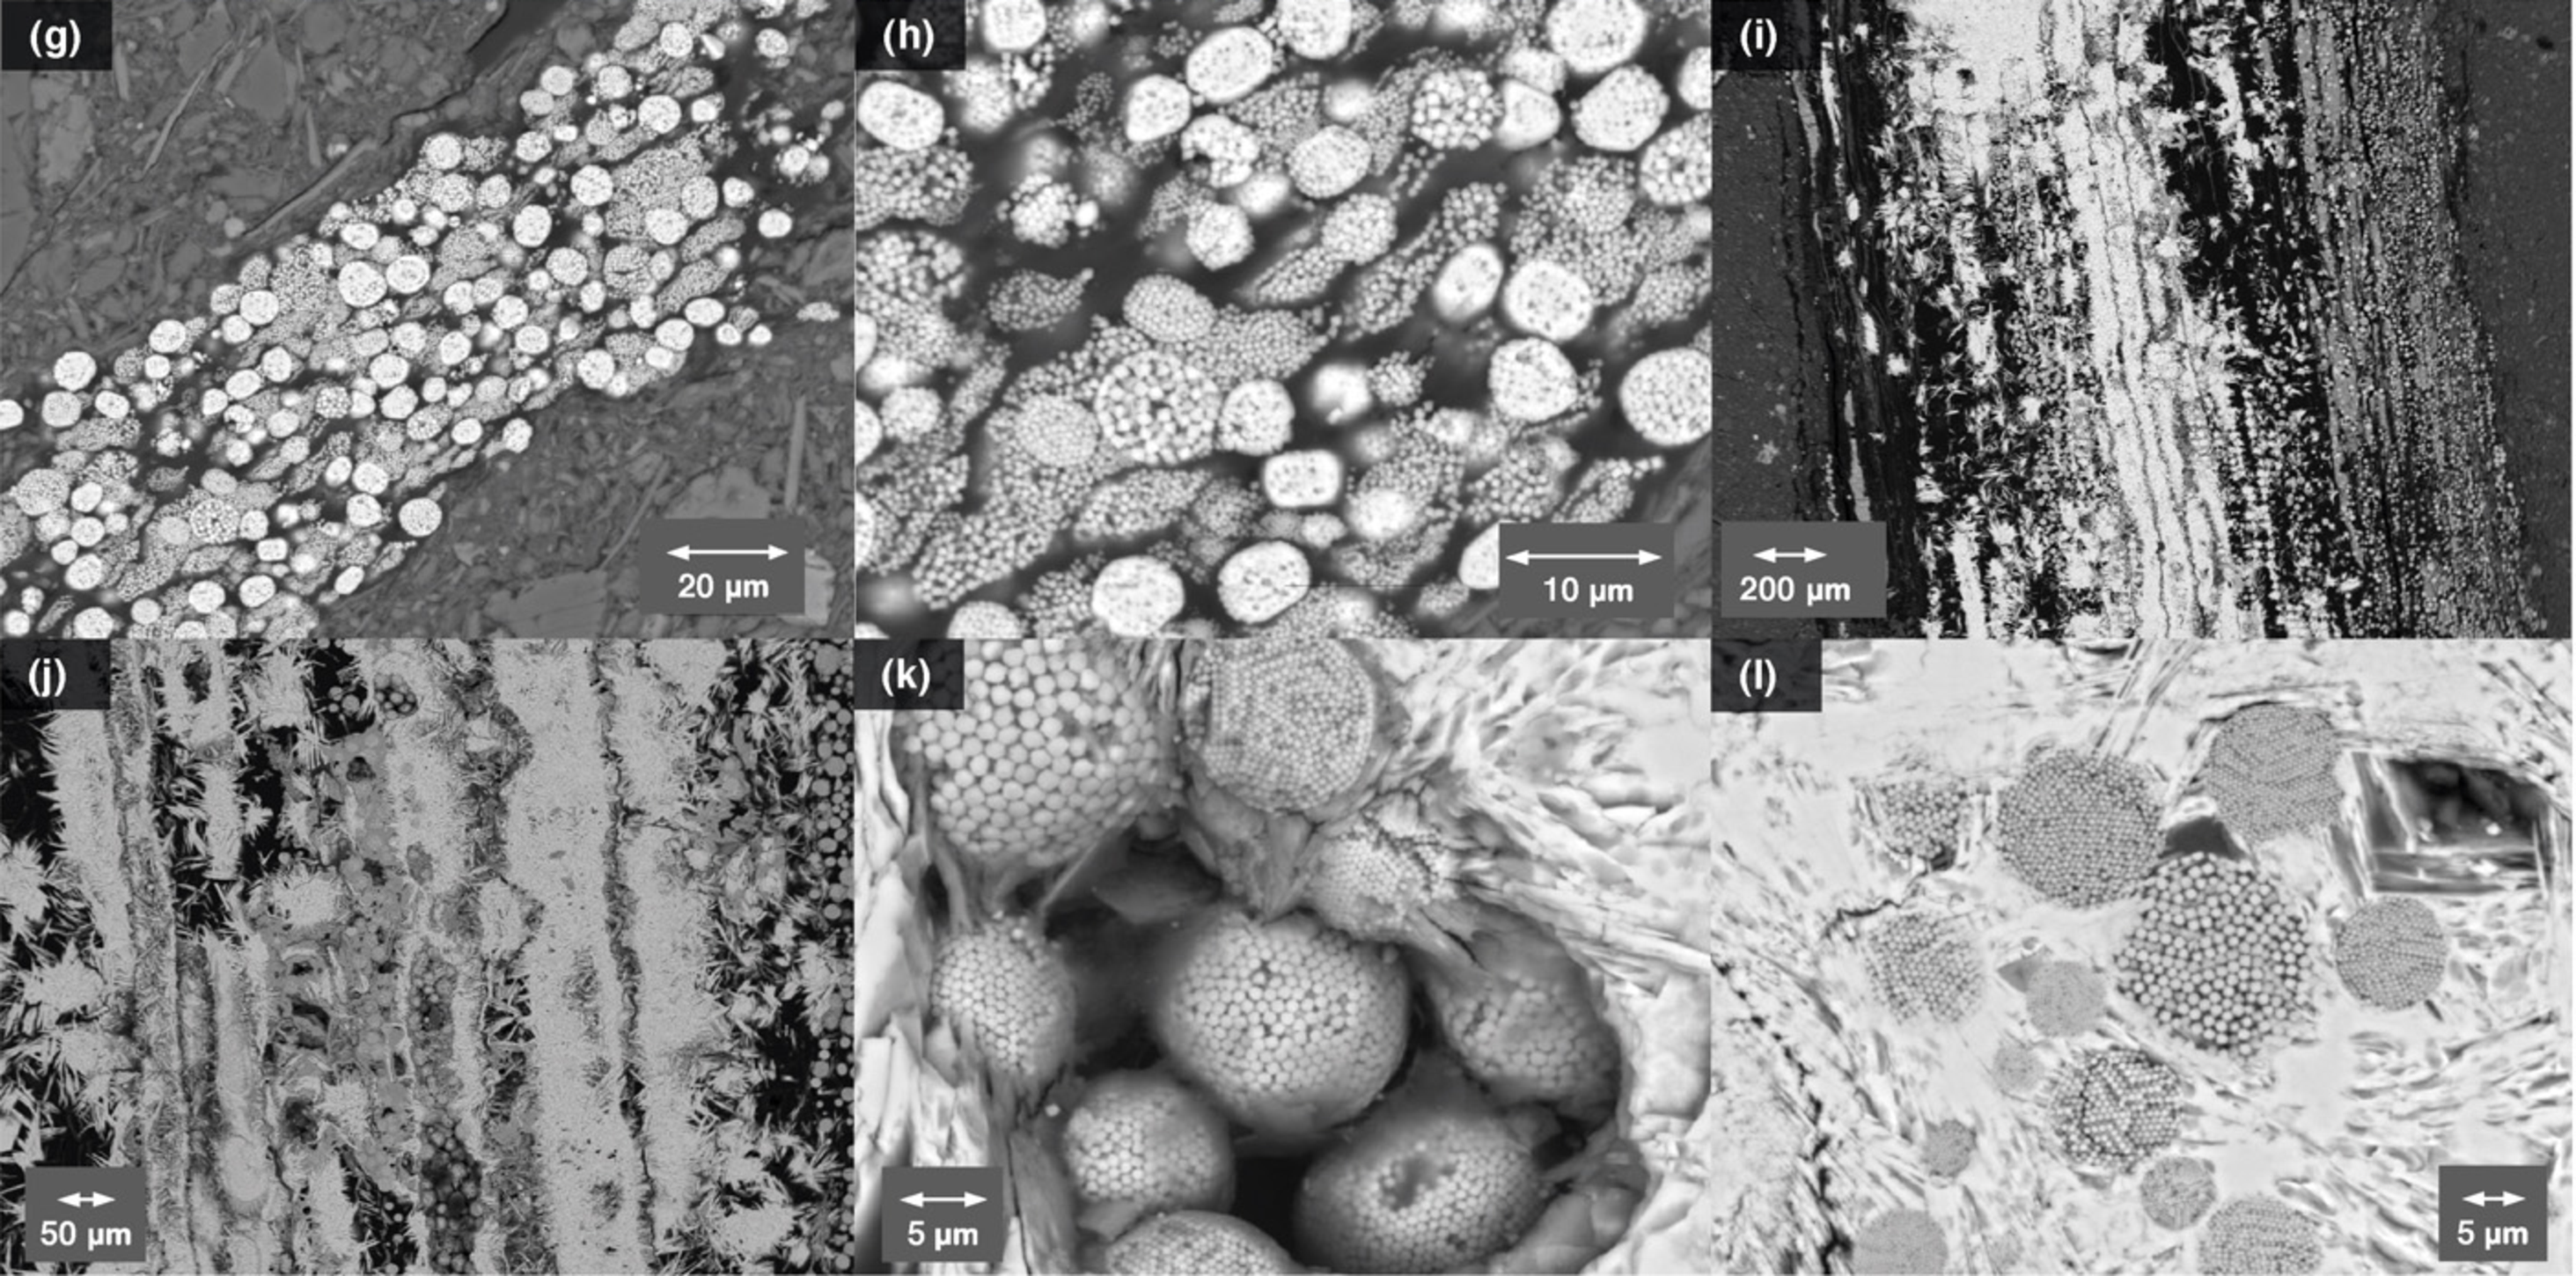
\includegraphics[width=\textwidth]{intro/figs/greigite_framboids.pdf}
\caption[SEM images of framboidal greigite]{SEM images at progressively higher magnification of framboidal greigite in sedimentary rocks. Greigite is the finer-grained phase and pyrite the coarser. (After \citet{Roberts2015}).}
\label{intro_01}
\end{figure}
\par

Given the unstable nature of greigite and the difficulties to produce synthetic samples, numerical investigations have the potential to answer important questions about greigite that can have great impact on magnetic hydrocarbon exploration and environmental magnetic studies. In this thesis, numerical models are employed to address some open questions about the iron sulphide greigite.\par

In Chapter \ref{ch:res-1}, the zero-field size dependence of the magnetic structure of greigite is investigated for a variety of naturally occurring shapes via a micromagnetic finite element method (FEM). A nudged elastic-band (NEB) method is used to calculate minimal action paths between minimal energy states for a variety of shapes and sizes. This allows calculation of the stability of a magnetisation, with implications for palaeomagnetic studies.\par

A simplified numerical model is developed in Chapter \ref{ch:res-2} to study the hysteresis of small greigite grains in a SD state. A spherical magnetic particle is essentially treated as a magnetic dipole; a gradient method is used to find the energy minimum in an applied field. This model is used to study the first-order reversal curve (FORC) diagrams produced by randomly oriented dispersions of non-interacting SD greigite (and iron as another interesting application).\par

A micromagnetic model is used to study the FORC response of randomly oriented non-interacting particle dispersions of greigite with a variety of sizes in Chapter \ref{ch:res-3}. The FORC signal of dispersions of particles with non-uniform single-vortex (SV) magnetisations is investigated. This model results in heuristics for interpretation of FORC signals when the magnetisations are carried by particles in the SV state.\par

The effects of strong inter-particle magnetostatic interactions on the FORC response is investigated in Chapter \ref{ch:res-4}. Framboidal geometries are used to study the FORC signal of randomly oriented dispersions of framboidal greigite. The signal is identified with consequences for the interpretation of FORC diagrams of greigite-rich sediments.\par

\section{The iron sulphide greigite}
summary of greigite properties Roberts 2011

summary of greigite formation and preservation

\section{Micromagnetics}
The micromagnetic formalism, equations

\section{Finite-element method}
The finite element formulation of micromagnetism

%----------------------------------
\renewcommand\bibname{{References}}
\bibliographystyle{elsarticle-harv}
\bibliography{references}

